\chapter{Prediction Models for SOSAA} \label{txt:prediction-chapter}

This project explores the feasibility of training a prudent Response Surface Model on SOSAA model runs using the Icarus architecture (see \Cref{txt:icarus-rsm}). The Icarus RSM consists of an out-of-distribution detector, a prediction model, and an uncertainty quantifier. While \Cref{txt:ood-detection-chapter} has explored different OOD detection methods, the following chapter analyses different prediction models. Afterwards, \Cref{txt:uncertainty-chapter} delves into quantifying the uncertainty of the model predictions. In the following explorations, we use the trajectory dataset introduced in \Cref{txt:sosaa-data-chapter}. It contains all external inputs to SOSAA, which we use as model input data.

In particular, we explore how well several simple machine-learning models can predict the $\log_{10}(CCN)$ target variable for the trajectory on which they are trained. We further analyse if they can generalise to other trajectories. Each model is trained on $75\%$ of the data from the 15.05.2018 19:00 UTC trajectory. Typically, this $75\%$ large training data set would be obtained using independent and identically distributed random sampling. However, we instead introduce a clumping method in \Cref{txt:clumped-train-test-split} which ensures that adjacent time steps are more likely to be both in the training or both in the test set. Next, \Cref{txt:model-criteria} introduces the experimental setup and visualisations we use in this chapter to evaluate the models we train in \Cref{txt:model-evaluation}. Finally, \Cref{txt:model-conclusions} closes with some brief recommendations on choosing a prediction model for the Icarus RSM.

\section{Clumped Train-Test Data Splits} \label{txt:clumped-train-test-split}

In machine learning, datasets are usually split into disjoint training and test datasets using independent and identically distributed (iid) random samples. For the time series SOSAA trajectory data, however, such an iid split would spread out the training set samples such that any test data point is likely surrounded by several training samples between which a model can simply interpolate. We introduce clumped train-test dataset splits to discourage the models from relying on such spatiotemporal memory alone.

In our experiments, we group all samples from a single time step together, which can either be all in the training or all in the test set. Our sampling method can be applied to any such atomic sample groupings, which may also contain only one sample each. Whether one group (time step) belongs to the training or test set is \textit{not} independent of the previous group's choice. In particular, we define a clumping factor $clump \in [0.0; 1.0]$ that determines the strength of this dependence. While $clump = 0.0$ produces an iid split of the groups, $clump = 1.0$ randomly puts all samples into either the training or test set.

\begin{multicols}{2}
    \noindent To split a dataset s.t. the fraction of training samples goes to $P(\texttt{train}) = p$, we introduce the following two-state Markov chain through its transition probabilities:
    \begin{enumerate}
        \item $P(\texttt{train} \rightarrowtail \texttt{train}) = a = 1 - (1-p) \cdot (1 - clump)$
        \item $P(\texttt{train} \rightarrowtail \texttt{test}) = b = 1-a$
        \item $P(\texttt{test} \rightarrowtail \texttt{train}) = c = (1-a) \cdot \frac{p}{1-p}$
        \item $P(\texttt{test} \rightarrowtail \texttt{test}) = d = 1-c$
    \end{enumerate}
    For $clump = 0.0$, $P(\texttt{train} \rightarrowtail \texttt{train}) = P(\texttt{test} \rightarrowtail \texttt{train}) = p$ and $P(\texttt{train} \rightarrowtail \texttt{test}) = P(\texttt{test} \rightarrowtail \texttt{test}) = 1-p$, i.e. the transition probabilities are state-independent of the current state, and the Markov chain produces iid samples as desired.
    \begin{figure}[H]
        \centering
        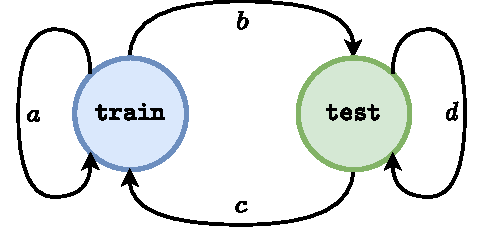
\includegraphics[width=0.49\textwidth]{prediction/figures/clumped-train-test.pdf}
        \caption[Clumped train-test split Markov chain]{Diagram of a two-state Markov chain that can produce a train-test split with varying clumping.}
        \label{fig:clumped-train-test}
    \end{figure}
\end{multicols}

\noindent For $clump = 1.0$, $P(\texttt{train} \rightarrowtail \texttt{train}) = P(\texttt{test} \rightarrowtail \texttt{test}) = 1$ and $P(\texttt{train} \rightarrowtail \texttt{test}) = P(\texttt{test} \rightarrowtail \texttt{train}) = 0$, i.e. the Markov chain gets stuck in the state it was initialised in. For the general case, we show that the Markov chain reaches its steady state of $P(\texttt{train}) = p$ and $P(\texttt{test}) = 1-p$, i.e. applying the Markov chain's transition matrix does not change the steady state:

\begin{equation*}
    \begin{split}
        \begin{bmatrix}
            P_{steady}(\texttt{train}) & P_{steady}(\texttt{test})
        \end{bmatrix} &\times \begin{bmatrix}
            P(\texttt{train} \rightarrowtail \texttt{train}) & P(\texttt{train} \rightarrowtail \texttt{test}) \\
            P(\texttt{test} \rightarrowtail \texttt{train}) & P(\texttt{test} \rightarrowtail \texttt{test})
        \end{bmatrix} \\
        &= \begin{bmatrix}
            p & 1-p
        \end{bmatrix} \times \begin{bmatrix}
            a & b \\
            c & d
        \end{bmatrix} \\
        &= \begin{bmatrix}
            ap + c(1-p) && bp + d(1-p)
        \end{bmatrix} \\
        &= \begin{bmatrix}
            ap + (1-a) \cdot \frac{p}{1-p} \cdot (1-p) && (1-a)p + (1-c)(1-p)
        \end{bmatrix} \\
        &= \begin{bmatrix}
            ap + p - ap && (1-a)p + (1-((1-a) \cdot \frac{p}{1-p}))(1-p)
        \end{bmatrix} \\
        &= \begin{bmatrix}
            p && (1-a)p + (1-p) - (1-a)p
        \end{bmatrix} \\
        &= \begin{bmatrix}
            p && 1-p
        \end{bmatrix} = \begin{bmatrix}
            P_{steady}(\texttt{train}) & P_{steady}(\texttt{test})
        \end{bmatrix}
    \end{split}
\end{equation*}

\noindent In practice, a clumped train-test-split sampler can be implemented as shown in \Cref{exe:clumped-train-test}.

\begin{listing}[H]
    \capstart % manually apply hypcap
    \begin{minted}[linenos,escapeinside=@@]{python}
import numpy as np
    
def train_test_split(X, Y, rng, p_train=0.75, clump=0.0):
    TRAIN, TEST = 0, 1

    # Pre-calculate the transition probabilities
    p_train_to_train = 1 - (1-p_train)*(1-clump)
    p_test_to_train = (1-p_train_to_train) * p_train/(1-p_train)
    p_to_train = (p_train_to_train, p_test_to_train)

    # Initialise the first Markov chain to a random state
    # Note: If clump=1.0, all samples are in either the training
    #       or the test set, according to this initial state
    mc_states = np.zeros(shape=len(X), dtype=int)
    mc_states[0:1] = TRAIN if rng.u01() < P_train else TEST

    # Follow the Markov chain transitions
    for i in range(1, len(X)):
        mc_states[i] = TRAIN if rng.u01() < P_to_train[mc_states[i-1]] else TEST

    # Split X and Y into training and test set
    X_train, X_test = X[np.nonzero(mc_states == TRAIN)], X[np.nonzero(mc_states == TEST)]
    Y_train, Y_test = Y[np.nonzero(mc_states == TRAIN)], Y[np.nonzero(mc_states == TEST)]

    return X_train, X_test, Y_train, Y_test
    \end{minted}
    \caption[Clumped train-test-split procedure]{Example Python implementation of a train-test-split function with clumping. The \texttt{numpy} arrays \texttt{X} and \texttt{Y} are randomly partitioned using a \texttt{rng}. Further shuffling of the returned datasets is omitted for brevity.}
    \label{exe:clumped-train-test}
\end{listing}

\section{Methods for Evaluating Prediction Models} \label{txt:model-criteria}

The models in this chapter are evaluated using three plots each, which span one row. The left plot shows how well each model can reproduce the CCN concentration time-height profile for its training trajectory. These plots are similar to \Cref{fig:six-trajectories-ccn} as they plot the CCN concentration on the y-axis against trajectory time on the x-axis, which repeats the timeline colour-coding from \Cref{fig:six-trajectories-maps}. In addition to labels \cite{mpl-label-lines-2022}, they also again use colours to encode the height of each layer. For better readability, only every sixth layer is shown, and the layers are distributed across five vertically-stacked subplots. The true CCN concentration is plotted as a light-and-dark dotted line, while the predicted CCN concentration is drawn as a solid height-coloured line. The grey shading in the background across some time periods indicates that these time steps were included in the training data set. Thus, the model is expected to perform very well on the shaded parts but make more mistakes in the unshaded regions. Note again that the models make predictions independently for each time step and height level.

The middle plot broadens the analysis from one trajectory to all six from \Cref{txt:six-trajectories}. Here, the true CCN concentration on the x-axis is plotted against the predicted CCN concentration on the y-axis. Note that this second plot only captures the performance on unseen data points from each trajectory's test set. If a model were a perfect predictor, all of its predictions would lie on a diagonal, which is indicated by a black-and-white line, and points above this line indicate overpredictions. If the model reports any uncertainties, the points use the CET-L8 colour map \cite{color-cet-2015, color-cet-2023} to represent the model's uncertainty in the prediction. Low-uncertainty points are shown in dark blue, while high-uncertainty points are in yellow. The range and colour-coding of the prediction uncertainty are shown on the right y-axis of the plot. Finally, the plot also contains the \textbf{M}ean \textbf{S}quared \textbf{E}rror and \textbf{M}ean \textbf{A}bsolute \textbf{E}rror and $R^2$ scores, all calculated in $\log_{10}(CCN)$ space. Note that while lower errors are better, the $R^2$ score of a model is $1.0$ at best but can be arbitrarily negative.

Last but not least, the third plot on the right mirrors the middle plot but examines the performance of a model that is trained on the training data from all six trajectories and tested on the testing data from all six trajectories. Note that all training and test data sets remain disjoint. This final plot provides an upper limit for how much a method can learn if given access to diverse training data that is similar to the test data. Thus, it serves as a comparison with the generalisation performance in the middle plot.

\section{Comparison of Prediction Models for SOSAA} \label{txt:model-evaluation}

First up, \Cref{fig:linear-tree-models} examines the performance of linear models (see \Cref{txt:linear-model}) and Decision Trees (see \Cref{txt:ensembles-decision-tree-random-forest}). These two methods only produce a single point-prediction and thus do not assign uncertainty to their predictions out of the box. While the linear model mostly performs reasonably well when predicting for the data it was trained on, excluding the second-highest height level shown, it has significant prediction errors for the test data. Hence it is unsurprising that the linear model fails entirely when generalising to a bigger test set. In particular, it predicts absurd CCN concentration values. However, if given access to a more diverse training set that is similar to its test set, the linear model can produce reasonable predictions.

\begin{figure}[H]
    \begin{subfigure}
    \centering
    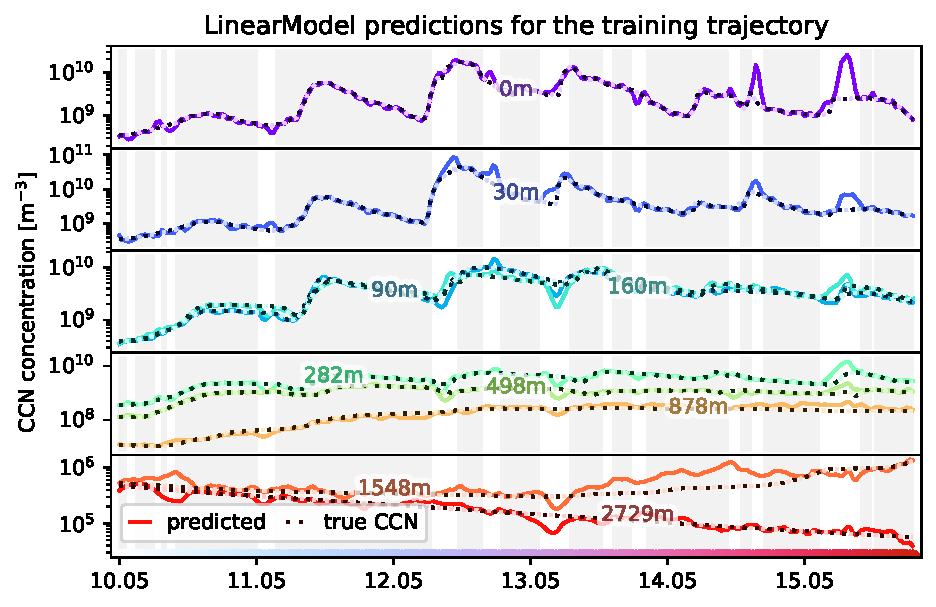
\includegraphics[width=0.4\textwidth]{prediction/figures/models/linearmodel-training-prediction.pdf}
    \end{subfigure}
    \begin{subfigure}
    \centering
    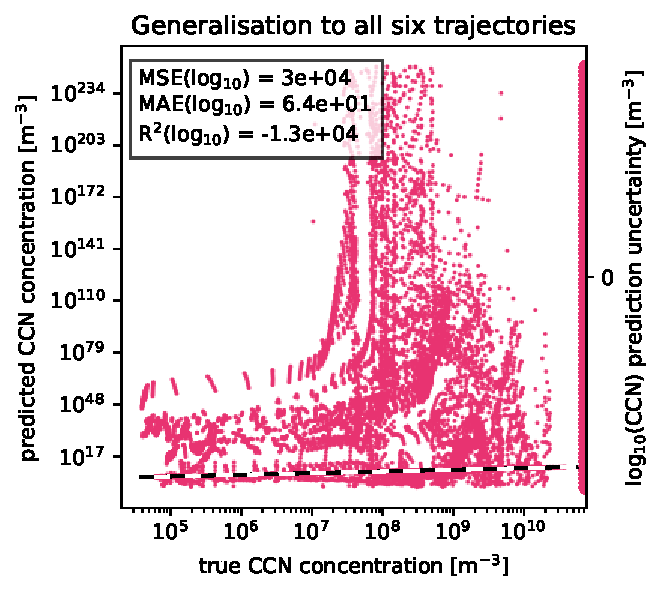
\includegraphics[width=0.275\textwidth]{prediction/figures/models/linearmodel-test-generalisation.pdf}
    \end{subfigure}
    \begin{subfigure}
    \centering
    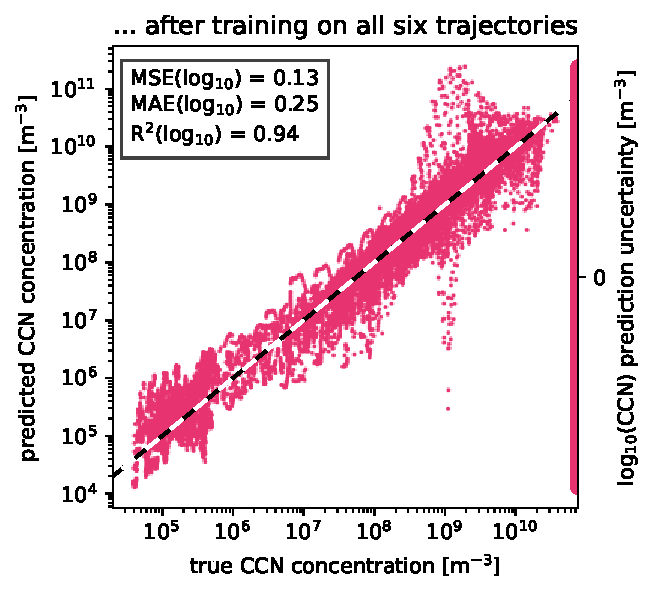
\includegraphics[width=0.275\textwidth]{prediction/figures/models/linearmodel-test-prediction.pdf}
    \end{subfigure}
   
    \begin{subfigure}
    \centering
    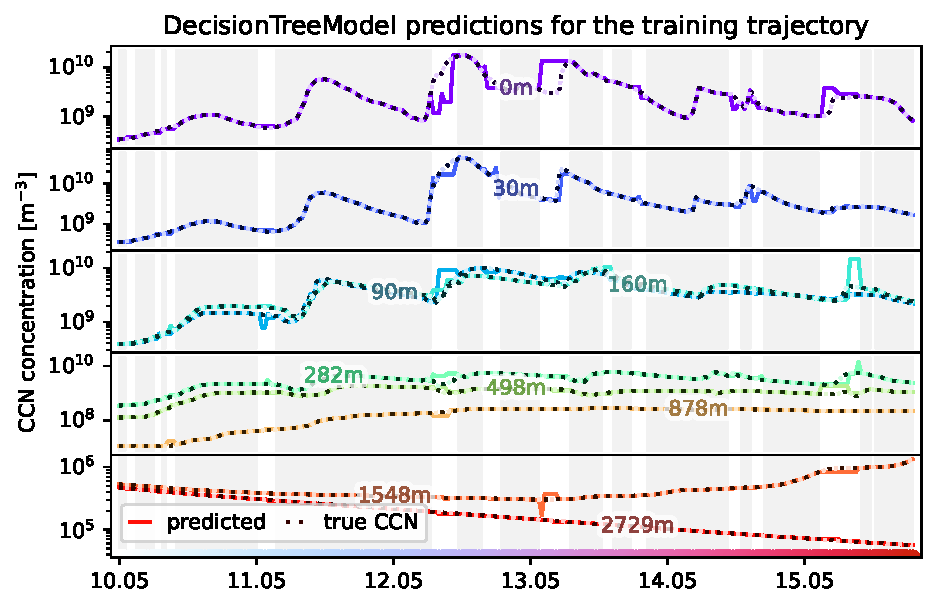
\includegraphics[width=0.4\textwidth]{prediction/figures/models/decisiontreemodel-training-prediction.pdf}
    \end{subfigure}
    \begin{subfigure}
    \centering
    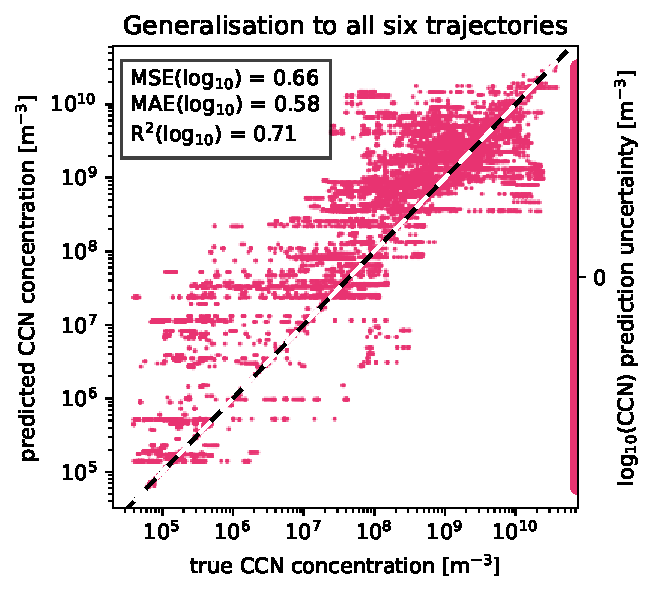
\includegraphics[width=0.275\textwidth]{prediction/figures/models/decisiontreemodel-test-generalisation.pdf}
    \end{subfigure}
    \begin{subfigure}
    \centering
    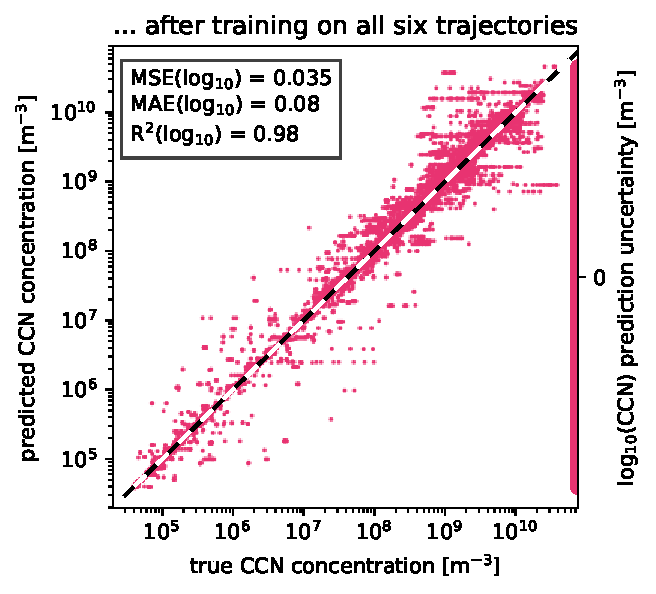
\includegraphics[width=0.275\textwidth]{prediction/figures/models/decisiontreemodel-test-prediction.pdf}
    \end{subfigure}
   
    \vspace{-1em}
    \caption[Predictive Performance of Linear models and Decision Trees]{Comparison of the predictive performance (see \Cref{txt:model-criteria}) of Linear models and Decision Trees on the full training trajectory (left), their generalisation to cross-trajectory test data (middle), and performance limit when trained on all six trajectories from \Cref{txt:six-trajectories}. Neither of the models reports uncertainties.}
    \label{fig:linear-tree-models}
\end{figure}

\noindent Decision Trees often match the true CCN concentration more closely. However, their rule-based and blocky prediction patterns become apparent in some snappy misprediction jumps on the test set. Still, they perform better at generalisation, though this is primarily because they do not predict outrageous CCN concentrations.

\newpar Next, \Cref{fig:bayesian-gp-models} looks at the performance of Sparse Bayesian models and Gaussian Processes (see \Cref{txt:gaussian-process}). The Sparse Bayesian models use a Gaussian prior over the parameters of a linear regression model that takes parameter relevance into account \cite{sparse-bayesian-1996}. For simplicity, we treat them as linear models that also predict their posterior uncertainty. Please refer to \textcite{sparse-bayesian-1996} for further information on the method. While these models perform slightly better than linear models, they also predict absurd CCN concentrations. However, they at least also assign the highest uncertainty to the points that they predict with the greatest error.

\begin{figure}[H]
    \begin{subfigure}
    \centering
    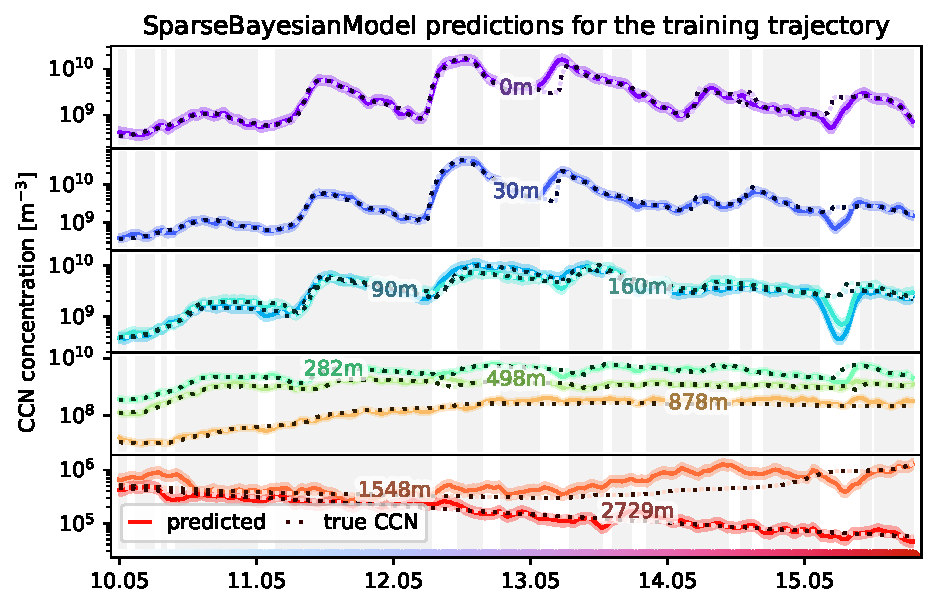
\includegraphics[width=0.4\textwidth]{prediction/figures/models/sparsebayesianmodel-training-prediction.pdf}
    \end{subfigure}
    \begin{subfigure}
    \centering
    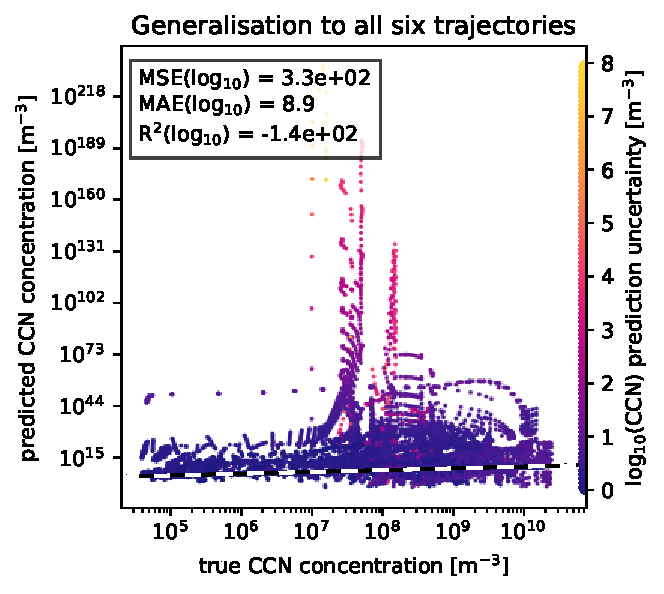
\includegraphics[width=0.275\textwidth]{prediction/figures/models/sparsebayesianmodel-test-generalisation.pdf}
    \end{subfigure}
    \begin{subfigure}
    \centering
    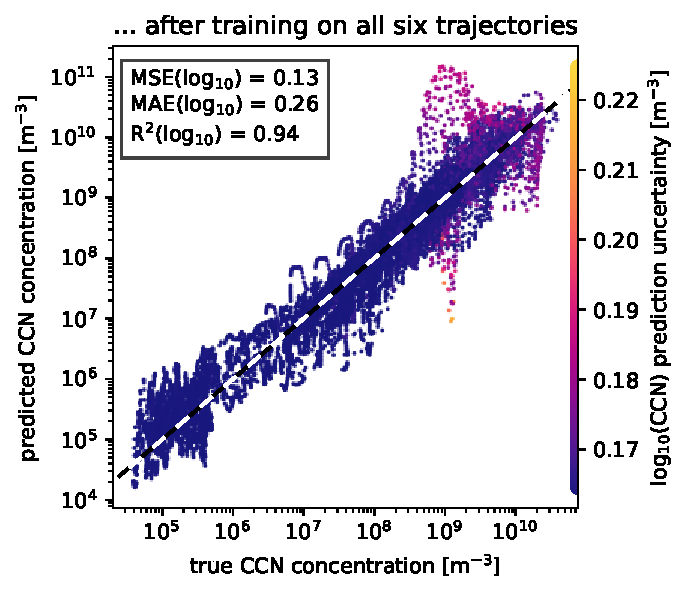
\includegraphics[width=0.275\textwidth]{prediction/figures/models/sparsebayesianmodel-test-prediction.pdf}
    \end{subfigure}
   
    \begin{subfigure}
    \centering
    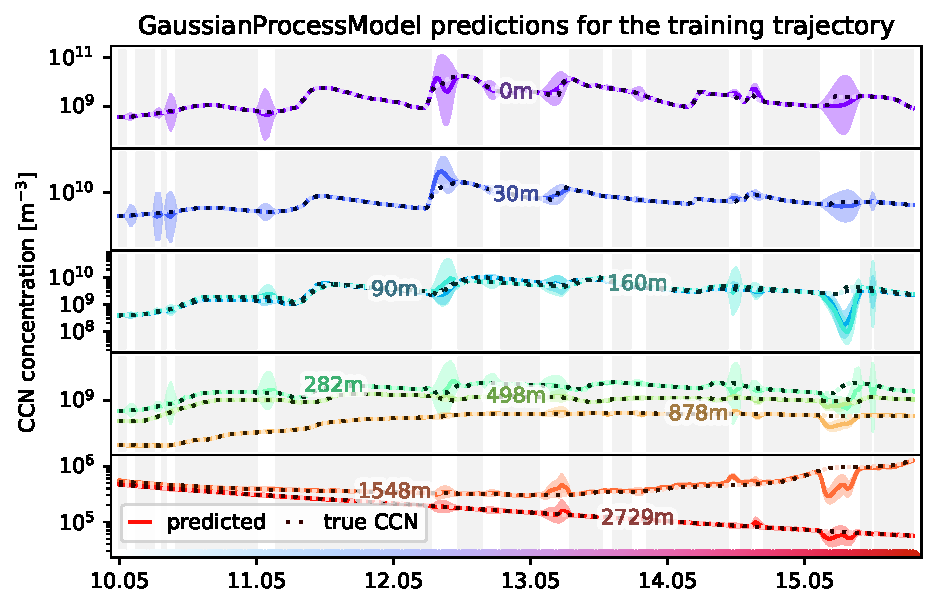
\includegraphics[width=0.4\textwidth]{prediction/figures/models/gaussianprocessmodel-training-prediction.pdf}
    \end{subfigure}
    \begin{subfigure}
    \centering
    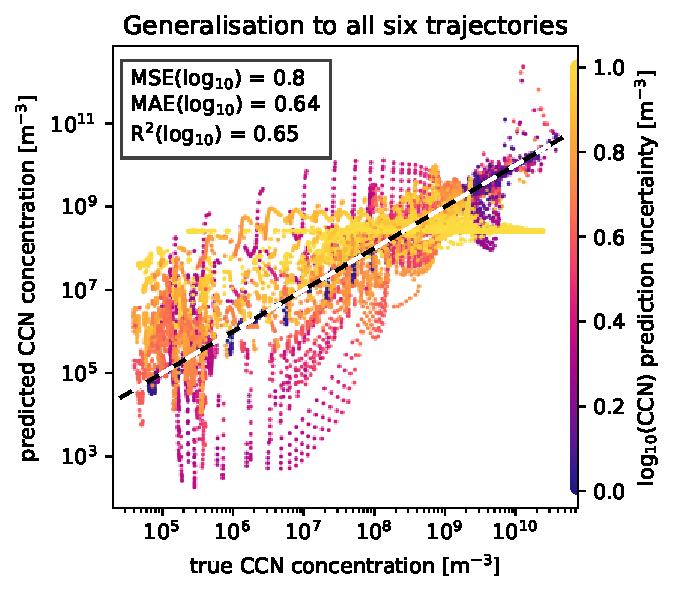
\includegraphics[width=0.275\textwidth]{prediction/figures/models/gaussianprocessmodel-test-generalisation.pdf}
    \end{subfigure}
    \begin{subfigure}
    \centering
    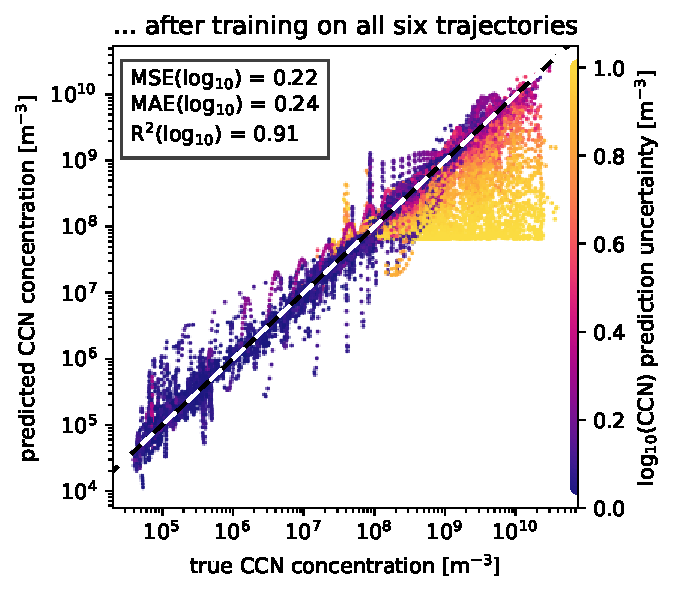
\includegraphics[width=0.275\textwidth]{prediction/figures/models/gaussianprocessmodel-test-prediction.pdf}
    \end{subfigure}
   
    \vspace{-1em}
    \caption[Predictive Performance of Sparse Bayesian models and Gaussian Processes]{Comparison of the predictive performance (see \Cref{txt:model-criteria}) of Sparse Bayesian models and Gaussian Processes on the full training trajectory (left), their generalisation to cross-trajectory test data (middle), and performance limit when trained on all six trajectories from \Cref{txt:six-trajectories}. Both models report uncertainties.}
    \label{fig:bayesian-gp-models}
\end{figure}

\noindent Gaussian Processes have $\text{O}(N^3)$ complexity for $N$ training samples. Thus, faster approximations such as sub-sampling or Stochastic Variational GPs \cite{svgp-2013} are often used. For fairness, we still attempted to train the GPs on the full dataset despite the computational cost. When trained on the full data from a single trajectory with a combined radial basis function kernel and white noise kernel, GPs replicate the training data well and predict high uncertainty for the test data. Unfortunately, this meaningful uncertainty does not generalise well to unseen trajectories. Furthermore, training on all trajectories was only possible after subsampling the data to one-sixth. We thus do not further explore GP prediction models on larger datasets.

\newpar Following on, \Cref{fig:mlp-models} analyses the performance of Multi-Layer Perceptrons, which are simple fully-connected neural networks. In our experiments, they have three hidden layers with $128$ neurons each that use the ReLU activation function. These simple networks produce relatively smooth predictions that generalise to some test data whilst failing with high error for inputs such as the unshaded test period after May 15\textsuperscript{th}. When applied to new trajectories, the MLPs produce significant overpredictions that exceed physically realistic ranges. However, if trained on a more extensive and diverse training data set, MLPs can produce high-accuracy predictions.

\newpar How can we constrain the physically unrealistic predictions that the neural network makes on unseen trajectories? Before any of the models are trained, the target variable $\log_{10}(CCN)$ is standardised to have zero mean and unit variance. Thus, each model learns to predict data in the same range as a standard normal distribution, which is then scaled back up again before being output. We can more forcefully constrain the MLP to predict values from this domain by training the model to predict the percentile of a standard normal distribution. For instance, the following last-level activation function transforms any real-valued prediction $\hat{y} \in [-\inf; +\inf]$ into a normal-constrained prediction $\hat{y}' \sim \text{N}(0, 1)$ using the inverse error function:

\begin{equation*}
    \hat{y}' = \text{erf}^{-1} \left( \text{softsign}(\hat{y}) \right) \cdot \sqrt{2} \quad \text{where} \quad \text{softsign}(x) = \frac{x}{1 + |x|}
\end{equation*}

\noindent The second row of \Cref{fig:mlp-models} shows the MLP still does not generalise well despite sticking to physical ranges.

\begin{figure}[H]
    \begin{subfigure}
    \centering
    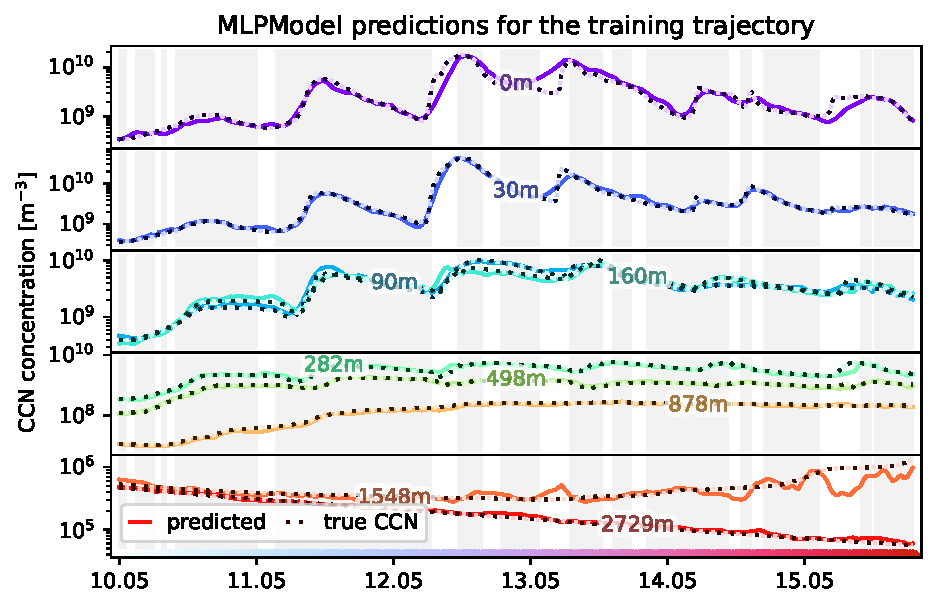
\includegraphics[width=0.4\textwidth]{prediction/figures/models/mlpmodel-training-prediction.pdf}
    \end{subfigure}
    \begin{subfigure}
    \centering
    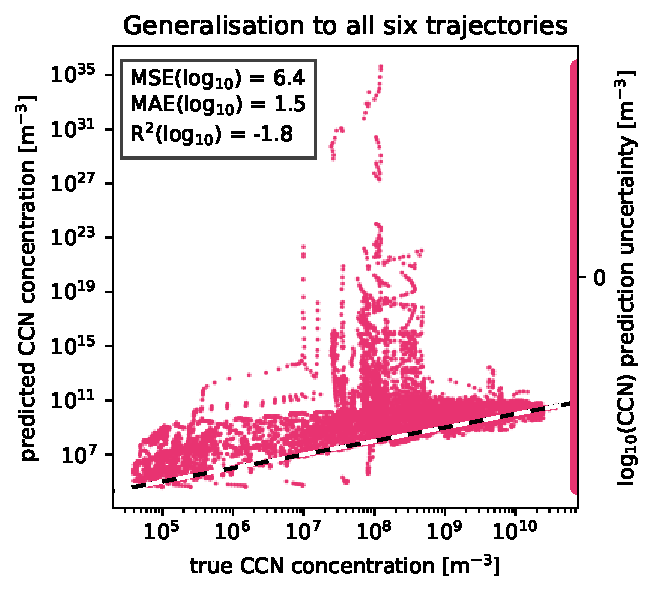
\includegraphics[width=0.275\textwidth]{prediction/figures/models/mlpmodel-test-generalisation.pdf}
    \end{subfigure}
    \begin{subfigure}
    \centering
    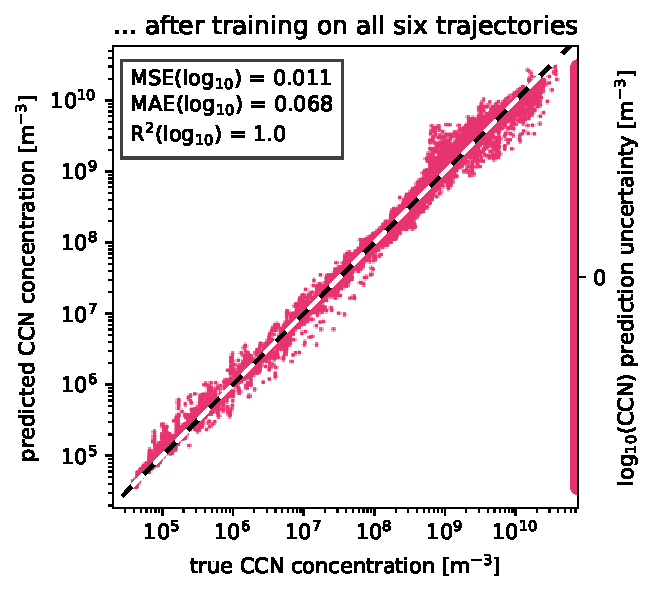
\includegraphics[width=0.275\textwidth]{prediction/figures/models/mlpmodel-test-prediction.pdf}
    \end{subfigure}

    \begin{subfigure}
    \centering
    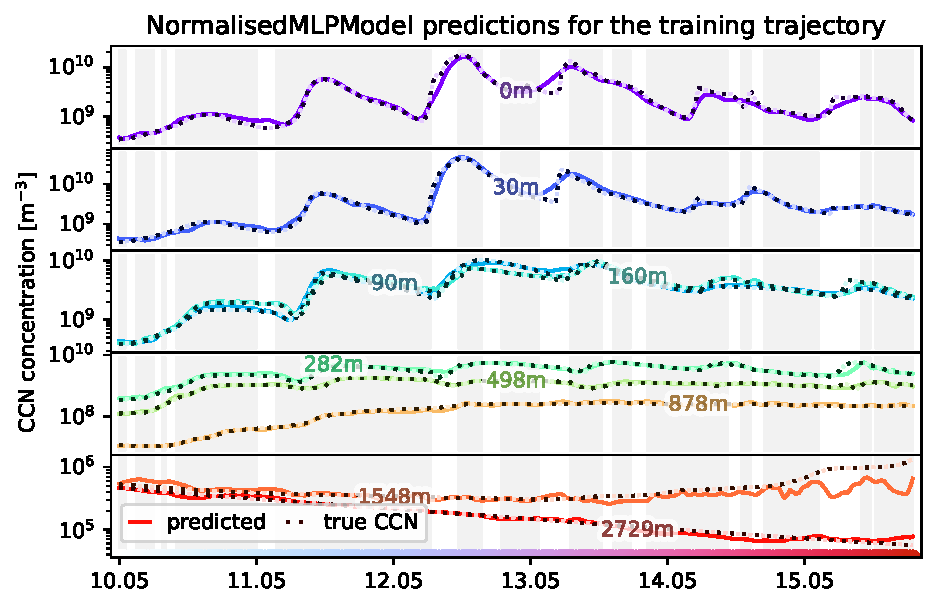
\includegraphics[width=0.4\textwidth]{prediction/figures/models/normalisedmlpmodel-training-prediction.pdf}
    \end{subfigure}
    \begin{subfigure}
    \centering
    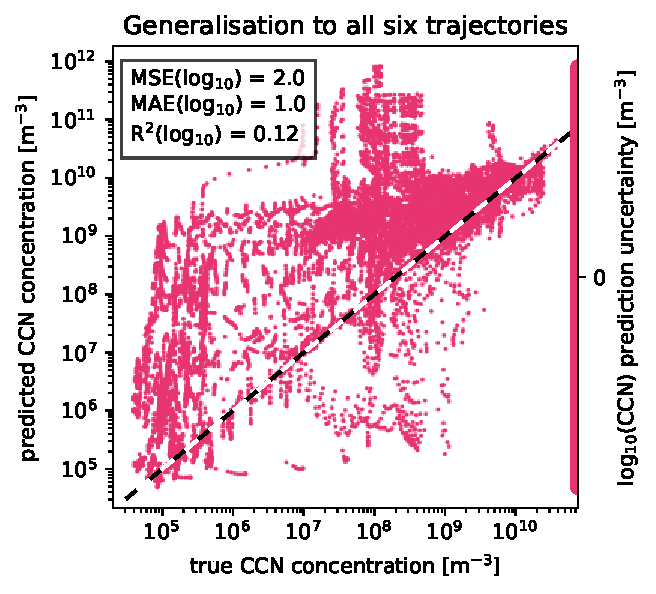
\includegraphics[width=0.275\textwidth]{prediction/figures/models/normalisedmlpmodel-test-generalisation.pdf}
    \end{subfigure}
    \begin{subfigure}
    \centering
    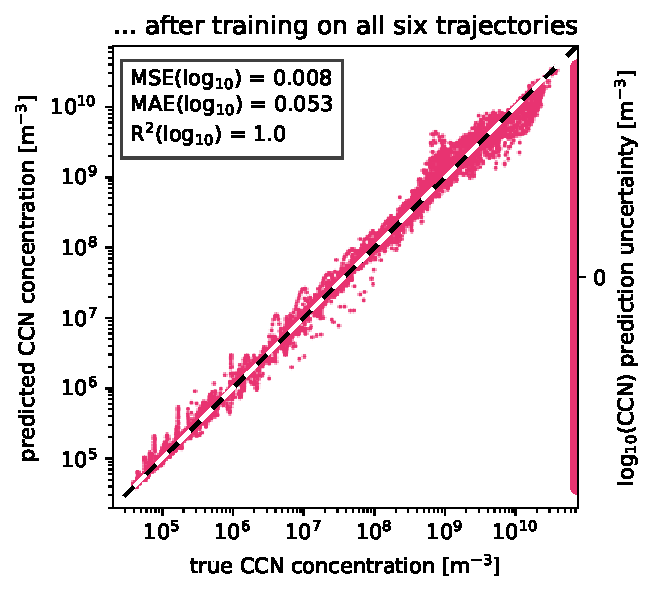
\includegraphics[width=0.275\textwidth]{prediction/figures/models/normalisedmlpmodel-test-prediction.pdf}
    \end{subfigure}

    \vspace{-1em}
    \caption[Predictive Performance of Multi-Layer Perceptrons]{Comparison of the predictive performance (see \Cref{txt:model-criteria}) of Multi-Layer Perceptrons, without and with forceful normalisation, on the full training trajectory (left), their generalisation to cross-trajectory test data (middle), and performance limit when trained on all six trajectories from \Cref{txt:six-trajectories}.}
    \label{fig:mlp-models}
\end{figure}

\noindent We continue by investigating Random Forests in the first row of \Cref{fig:rf-padre-rf-models}. As ensembles of decision trees, they have similar but slightly improved performance characteristics. During training, we only allow the random forests to look at one-third of the features at each split and require at least five examples per leaf node to discourage overfitting \cite{statistical-learning-2009}. While the RFs produce very accurate predictions on the training data, they have higher errors and higher ensemble uncertainty on the test data. However, this sensible uncertainty quantification does not seem to fully generalise to unseen trajectories.

\begin{figure}[H]
    \begin{subfigure}
    \centering
    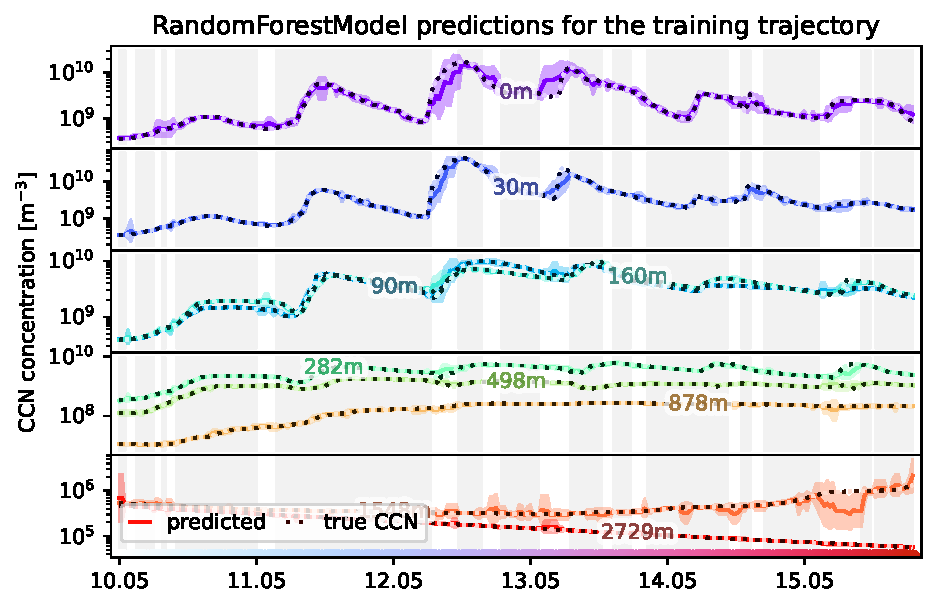
\includegraphics[width=0.4\textwidth]{prediction/figures/models/randomforestmodel-training-prediction.pdf}
    \end{subfigure}
    \begin{subfigure}
    \centering
    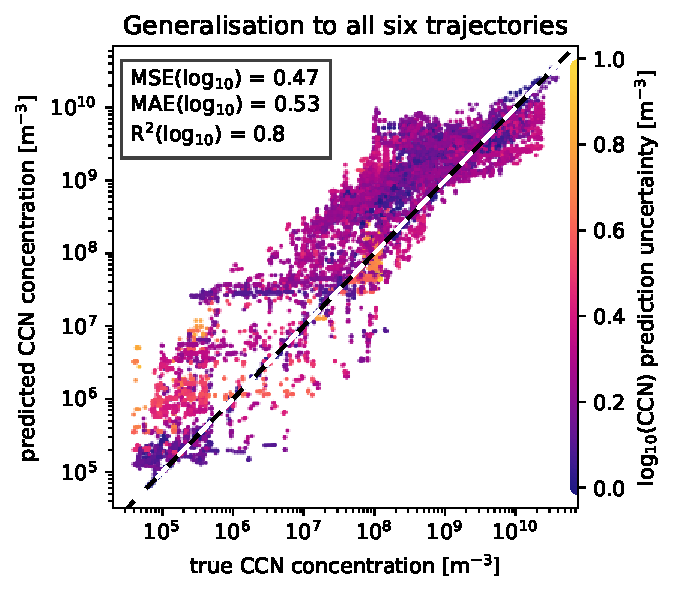
\includegraphics[width=0.275\textwidth]{prediction/figures/models/randomforestmodel-test-generalisation.pdf}
    \end{subfigure}
    \begin{subfigure}
    \centering
    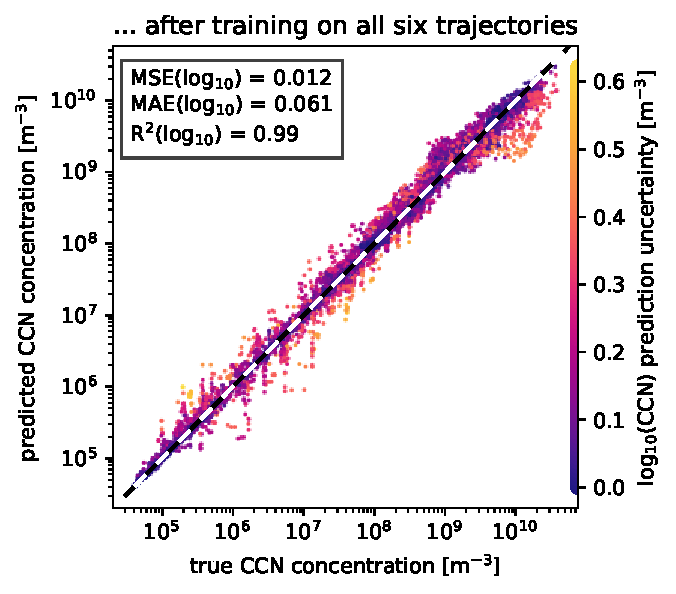
\includegraphics[width=0.275\textwidth]{prediction/figures/models/randomforestmodel-test-prediction.pdf}
    \end{subfigure}

    \begin{subfigure}
    \centering
    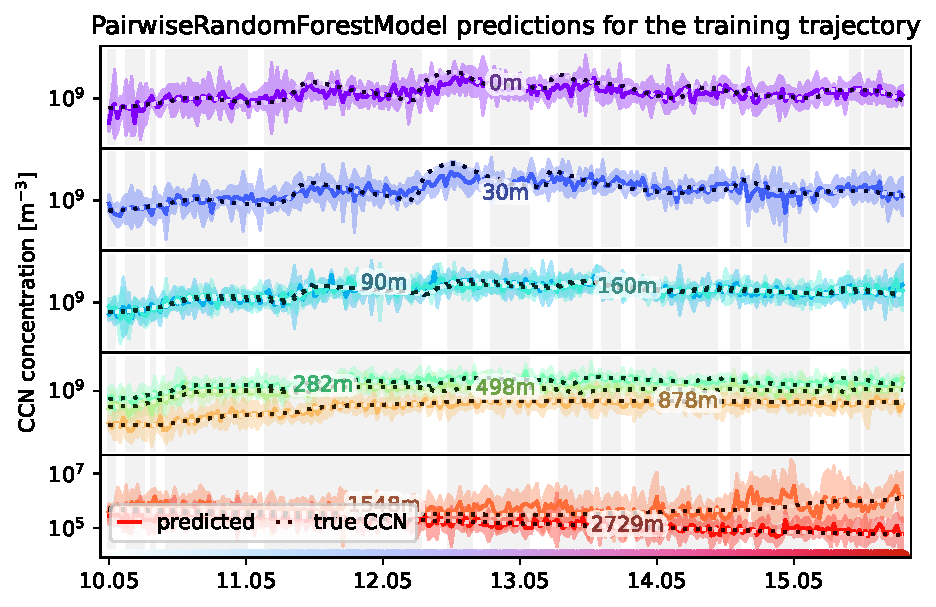
\includegraphics[width=0.4\textwidth]{prediction/figures/models/pairwiserandomforestmodel-training-prediction.pdf}
    \end{subfigure}
    \begin{subfigure}
    \centering
    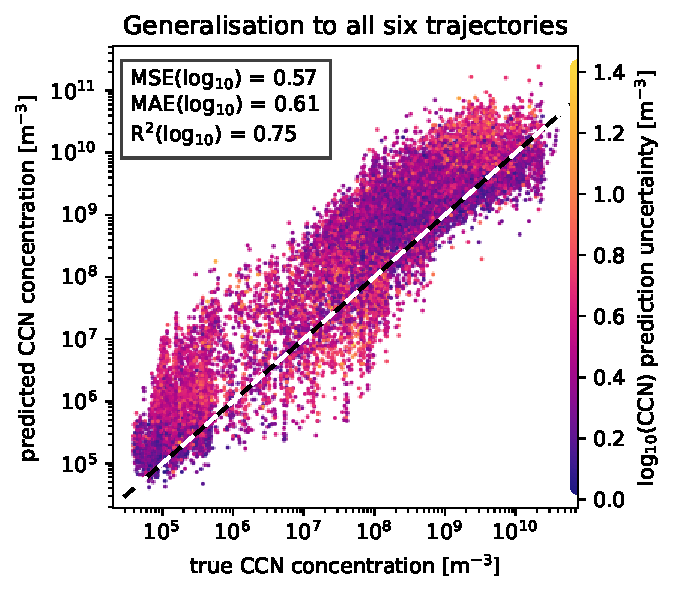
\includegraphics[width=0.275\textwidth]{prediction/figures/models/pairwiserandomforestmodel-test-generalisation.pdf}
    \end{subfigure}
    \begin{subfigure}
    \centering
    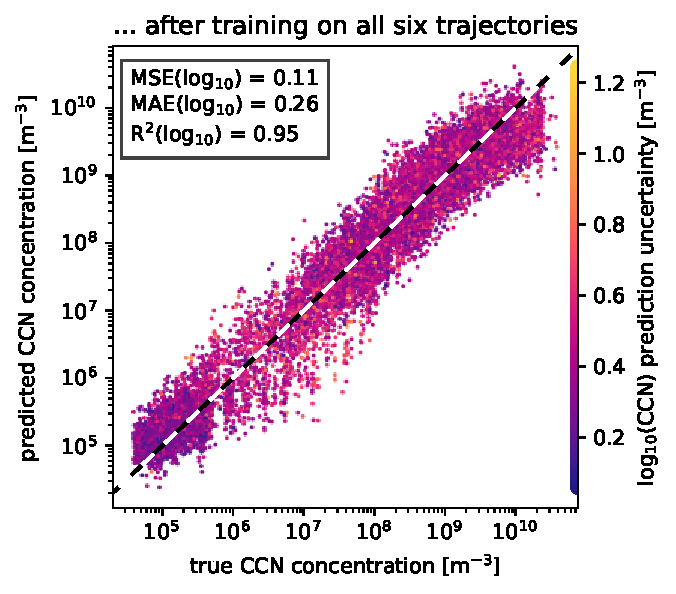
\includegraphics[width=0.275\textwidth]{prediction/figures/models/pairwiserandomforestmodel-test-prediction.pdf}
    \end{subfigure}

    \vspace{-1em}
    \caption[Predictive Performance of Random Forests and Pairwise Difference Regression with RFs]{Predictive performance (see \Cref{txt:model-criteria}) of Random Forest and of Pairwise Difference Regression using Random Forests \cite{padre-rf-2021} on the full training trajectory (left), their generalisation to cross-trajectory test data (middle), and performance limit when trained on all six trajectories from \Cref{txt:six-trajectories}.}
    \label{fig:rf-padre-rf-models}
\end{figure}

\noindent Finally, we also experiment with Pairwise Difference Regression, implemented using Random Forests, which is described in \Cref{txt:padre-rf}. PADRE-RF reports uncertainties by examining the spread of predictions for the differences for a random subset of anchor points in the training data set. The second row in \Cref{fig:rf-padre-rf-models} clearly shows that PADRE-RF produces very noisy predictions whose mean does not always perfectly hit the true CCN concentrations. Furthermore, the predictive uncertainty does not change significantly between the test and training data. The prediction performance of PADRE-RF is slightly worse than that of normal Random Forests when generalising to unseen trajectories. While the method's accuracy further improves when trained on all six trajectories, it does not reach the performance of the decision tree, random forest or MLP models (see \Cref{fig:mlp-models}). Furthermore, the uncertainty predictions from PADRE-RF do not appear to correlate with the prediction error. However, the range of its predictions seems to be slightly less biased than that of Random Forests. Thus, PADRE-RF is an architecture to investigate further, particularly for generalising to unseen data. However, it should not be used for uncertainty quantification and should be replaced by other methods if accuracy is more important than robust generalisation.

\section{Recommendations for Prediction Models} \label{txt:model-conclusions}

This chapter has focused on the second component of the Icarus RSM, prediction models. First, we introduced a method to produce clumped train-test dataset splits that can make it more difficult for models to overfit on time-series data. Afterwards, we evaluated the performance of several machine-learning methods as prediction models on the SOSAA trajectories dataset. From these experiments, we come to the following recommendations:

\begin{enumerate}
    \item Gaussian Processes can perform well and produce valuable uncertainty differences between training and unseen data. However, the $\text{O}(N^3)$ complexity slightly limits these benefits since larger datasets can only be used with approximation methods.
    \item Multi-Layer Perceptrons excel if they are fit on data from the same dataset but struggle with generalising to other trajectories even if their predictions are forcefully normalised to stay within a physically realistic domain.
    \item Random Forests are easy to apply and generally outperform the other methods. Even though Pairwise Difference Regression using Random Forests (PADRE-RF) produces highly uncertain predictions, it appears to generalise better to unseen trajectories.
\end{enumerate}

\noindent Given these conclusions, we decide to continue investigating Random Forests and PADRE-RF as prediction models for our Icarus RSM for the SOSAA model. It is important to remember, however, that no model is perfect but makes prediction mistakes even on in-distribution data. Therefore, \Cref{txt:uncertainty-chapter} follows up on this chapter and explores different methods for quantifying this prediction uncertainty.
